\chapter{Inflation due à un champ scalaire en évolution}

\lectureoverview{Une question laissée en suspens à la séance précédente fournit l’équation qui organise le cours,
\(\ddot\phi+3H\dot\phi=-V'(\phi)\) : qu’est-ce qui évolue, qu’est-ce qui exerce la force, et pourquoi l’expansion ressemble-t-elle à un frottement ? Nous dérivons d’abord l’équation dans une boîte fixe, puis dans une boîte en expansion. En la couplant à l’équation de Friedmann, on obtient le mécanisme de roulement lent, dans lequel un potentiel scalaire élevé et peu pentu entraîne une expansion presque exponentielle. L’inflation dilue les monopôles et lisse la géométrie ; à son terme, le réchauffement de l’Univers amorce le Big Bang chaud conventionnel. Reste alors une question inévitable : si l’inflation lisse si efficacement, d’où vient la structure ? Un calcul unidimensionnel de caustiques montre comment de minuscules variations de vitesse créent des nappes, des filaments et des nœuds, tandis que l’origine quantique de ces variations est laissée pour le cours suivant.}

\section{Qu’est-ce qui agit sur quoi ?}

La question d’ouverture rappelle l’équation
\begin{equation}
\ddot\phi+3H\dot\phi
=F(\phi)
=-\frac{dV}{d\phi}
\label{eq:c09-opening}
\end{equation}
et demande quel type de force \(F\) peut agir sur un champ. Cette question n’est pas accessoire. Pour y répondre, il faut reconstruire la mécanique du champ, ce qui nous amène à aborder l’inflation elle-même.

Un champ scalaire associe un nombre \(\phi(\mathbf x,t)\) à chaque point de l’espace-temps. Les champs électrique et magnétique portent de l’énergie ; un champ scalaire peut lui aussi en porter. Le champ dont nous avons besoin est hypothétique : aucun inflaton particulier n’a été identifié expérimentalement, et l’on ne connaît donc pas son énergie en fonction de la valeur du champ. Nous le représentons par une densité d’énergie potentielle indéterminée
\begin{equation}
V=V(\phi).
\label{eq:c09-potential}
\end{equation}
Différentes valeurs de \(\phi\) correspondent à différentes quantités d’énergie stockée par unité de volume physique.

Rien n’oblige \(\phi=0\) à avoir une énergie nulle. L’origine de l’espace des champs relève d’une convention, en particulier pour un champ encore inconnu, et décaler la coordonnée qui sert à désigner les valeurs du champ ne place pas nécessairement le minimum de \(V\) à l’origine. Le graphe de \(V(\phi)\) décrit les pentes et les hauteurs relatives, et non un point de départ privilégié pour le champ.

L’énergie potentielle est la part qui subsiste lorsque le champ est momentanément statique. Si le champ varie au cours du temps, il possède aussi une énergie cinétique. La quantité \(\dot\phi\) n’est pas la vitesse d’un objet dans l’espace ordinaire ; c’est le taux de variation de la valeur du champ, autrement dit une vitesse dans l’espace des champs. Une corde élastique fournit une analogie utile. Son déplacement est un champ défini sur un monde unidimensionnel, et un élément vibrant de la corde porte une énergie cinétique proportionnelle au carré de sa dérivée temporelle.

Le coefficient de ce carré peut être absorbé dans la définition du champ. Si l’on part de
\begin{equation}
\frac12 n^2\dot\phi^{\,2},
\end{equation}
alors le changement de variable
\begin{equation}
\chi=n\phi
\end{equation}
transforme le terme en \(\dot\chi^{\,2}/2\). On peut donc choisir un champ normalisé canoniquement et écrire, dans l’approximation homogène,
\begin{equation}
\rho_\phi=\frac12\dot\phi^{\,2}+V(\phi).
\label{eq:c09-rho-homogeneous}
\end{equation}
Il s’agit de normaliser la coordonnée dans l’espace des champs, et non d’affirmer que la masse d’une particule réelle a été fixée à l’unité.

\section{Mécanique dans une boîte fixe}

Considérons une petite boîte dans laquelle le champ est presque constant dans l’espace. Sa densité d’énergie a la même forme mathématique que l’énergie d’une particule de masse unité : énergie cinétique plus énergie potentielle. La densité lagrangienne associée porte le signe opposé devant le potentiel,
\begin{equation}
\mathcal L_\phi
=\frac12\dot\phi^{\,2}-V(\phi).
\label{eq:c09-lagrangian-density}
\end{equation}
L’analogie est mathématique. La coordonnée généralisée est la valeur du champ, et non la position spatiale d’une particule.

L’équation d’Euler--Lagrange est
\begin{equation}
\frac{d}{dt}
\left(
\frac{\partial\mathcal L_\phi}{\partial\dot\phi}
\right)
=
\frac{\partial\mathcal L_\phi}{\partial\phi}.
\label{eq:c09-el-fixed}
\end{equation}
Ici, la variable de vitesse est \(\dot\phi\), donc
\begin{equation}
\frac{\partial\mathcal L_\phi}{\partial\dot\phi}=\dot\phi,
\qquad
\frac{\partial\mathcal L_\phi}{\partial\phi}=-V'(\phi),
\end{equation}
on obtient
\begin{equation}
\ddot\phi=-V'(\phi)\equiv F(\phi).
\label{eq:c09-fixed-eom}
\end{equation}
La dérivée seconde est l’accélération de la coordonnée du champ, et la pente négative du potentiel en constitue la force.

\begin{figure}[htbp]
\centering
\includegraphics[width=0.88\textwidth]{lecture_09_figure_03.png}
\caption{La partie lisible du tableau montre \(V(\phi)\) dans l’équation de la boîte fixe \(\ddot\phi=-\partial V/\partial\phi\). L’expression d’Euler--Lagrange, en haut, est en partie coupée et masquée ; l’équation~\eqref{eq:c09-el-fixed} est donc reconstituée à partir de la dérivation plutôt que citée comme une transcription complète de l’image.}
\label{fig:c09-fixed-board}
\lectureframe{00:10:53.836}
\end{figure}

\begin{classroomqa}
\audiencequestion{Quelle est la force, et sur quoi agit-elle ?}
\lecturerresponse{C’est la valeur scalaire \(\phi\) qui évolue. La quantité \(-V'(\phi)\) est une force dans l’espace des champs : elle accélère la valeur du champ vers les énergies potentielles plus basses, tout comme \(-dV/dx\) accélère la coordonnée d’une particule. Ce n’est pas une nouvelle force vectorielle qui pousserait un corps matériel dans l’espace ordinaire. \lecturetimestamp{00:00:27--00:00:49; 00:10:41--00:11:29}}
\end{classroomqa}

Le champ complet peut dépendre de l’espace. Pour un champ scalaire canonique dans une géométrie en expansion spatialement plate, sa densité d’énergie locale comprend le terme
\begin{equation}
\rho_\phi
=
\frac12\dot\phi^{\,2}
+\frac{1}{2a^2}\lvert\nabla\phi\rvert^2
+V(\phi).
\label{eq:c09-rho-full}
\end{equation}
Nous négligeons le terme de gradient, car l’expansion étire les variations jusqu’à de grandes longueurs d’onde, rendant le champ presque uniforme dans la petite boîte. Cette approximation est justifiée par le contexte cosmologique ; elle ne nie pas l’existence possible d’ondes scalaires ou d’ondulations spatiales.

\section{La boîte en expansion}

La première dérivation répond à la question d’ouverture, mais ce n’est pas encore la dérivation cosmologique. Les équations~\eqref{eq:c09-rho-homogeneous} et \eqref{eq:c09-lagrangian-density} sont des densités. Le volume physique d’une boîte comobile unitaire est proportionnel à \(a^3(t)\), de sorte que son lagrangien est
\begin{equation}
L_\phi
=a^3(t)
\left[
\frac12\dot\phi^{\,2}-V(\phi)
\right].
\label{eq:c09-comoving-lagrangian}
\end{equation}
Dans une boîte statique, le facteur \(a^3\) n’aurait aucune importance. En cosmologie, il dépend du temps, et cette dépendance fournit le terme manquant.

\begin{figure}[htbp]
\centering
\includegraphics[width=0.88\textwidth]{lecture_09_figure_04.png}
\caption{À gauche, on distingue une courbe de potentiel dessinée à la main ; à droite apparaissent des fragments des expressions de l’énergie et du lagrangien. La courbe et le changement de signe sont clairement établis ; l’algèbre complète de l’équation~\eqref{eq:c09-comoving-lagrangian} provient de la dérivation orale, car l’enseignant masque une partie du tableau.}
\label{fig:c09-potential-board}
\lectureframe{00:13:26.528}
\end{figure}

En appliquant l’équation d’Euler--Lagrange à \(L_\phi\), on obtient
\begin{align}
\frac{d}{dt}\left(a^3\dot\phi\right)
&=-a^3V'(\phi), \label{eq:c09-a3-form}\\
a^3\ddot\phi+3a^2\dot a\,\dot\phi
&=-a^3V'(\phi),\\
\ddot\phi+3\frac{\dot a}{a}\dot\phi
&=-V'(\phi).
\end{align}
Avec \(H=\dot a/a\), le résultat est
\begin{equation}
\boxed{\ddot\phi+3H\dot\phi=-V'(\phi)}.
\label{eq:c09-hubble-friction}
\end{equation}
L’équation rappelée au début vient maintenant d’être dérivée, et non simplement évoquée.

\begin{figure}[htbp]
\centering
\includegraphics[width=0.96\textwidth]{lecture_09_figure_05.png}
\caption{La dynamique dans la boîte fixe à gauche et la correction due à l’expansion de la boîte à droite. Le tableau visible étaye le passage de \(d(a^3\dot\phi)/dt\) aux formes \(3\dot a/a\) et \(3H\) ; les membres de droite coupés sont complétés par l’équation~\eqref{eq:c09-a3-form}.}
\label{fig:c09-expanding-board}
\lectureframe{00:18:35.380}
\end{figure}

\begin{classroomqa}
\audiencequestion{Peut-on se représenter plus concrètement la force \(F\) ?}
\lecturerresponse{Représentons \(V(\phi)\) par un paysage dont la coordonnée horizontale est la valeur du champ. La pente détermine la force, \(F=-V'(\phi)\). Une forte pente descendante produit une grande force motrice dans l’espace des champs ; une pente douce, une force plus faible. Cette image aide à se représenter la coordonnée unidimensionnelle du champ ; elle ne décrit pas une colline située dans l’espace physique. \lecturetimestamp{00:18:26--00:19:18}}
\end{classroomqa}

\section{Frottement de Hubble et mouvement à vitesse limite}

Déplaçons le terme du milieu de l’équation~\eqref{eq:c09-hubble-friction} vers la droite :
\begin{equation}
\ddot\phi=-V'(\phi)-3H\dot\phi.
\end{equation}
Dans un Univers en expansion, \(H>0\), le deuxième terme s’oppose toujours à la vitesse du champ. Il se comporte donc comme une viscosité. Un rocher lâché dans du miel épais accélère d’abord, mais la force de traînée augmente avec sa vitesse jusqu’à ce qu’il atteigne une vitesse limite. Le moyen mnémotechnique \emph{\(H\) pour le miel} rappelle l’analogie, tandis que l’équation en donne le contenu exact. Si \(H\) varie avec le temps cosmique, la viscosité effective varie aussi, à la manière de la viscosité ordinaire lorsque la température change.

Lorsque le frottement domine l’inertie, \(\lvert\ddot\phi\rvert\ll3H\lvert\dot\phi\rvert\), et le champ approche rapidement
\begin{equation}
3H\dot\phi\simeq -V'(\phi),
\qquad
\dot\phi\simeq-\frac{V'(\phi)}{3H}.
\label{eq:c09-terminal}
\end{equation}
Un potentiel peu pentu fournit une faible force, tandis qu’un grand \(H\) produit une forte traînée. Ces deux effets rendent \(\dot\phi\) petit et rendent généralement la densité cinétique \(\dot\phi^2/2\) petite devant \(V\).

\begin{classroomqa}
\audiencequestion{Cette dérivation repose-t-elle sur le principe de moindre action ?}
\lecturerresponse{Oui. L’équation~\eqref{eq:c09-hubble-friction} s’obtient en rendant extrémale l’action construite à partir de l’équation~\eqref{eq:c09-comoving-lagrangian}. On peut aussi prendre l’équation du champ comme loi dynamique de départ, mais la dérivation variationnelle explique précisément pourquoi le volume en expansion contribue par le terme \(3H\dot\phi\). \lecturetimestamp{00:25:40--00:26:15}}
\end{classroomqa}

\begin{classroomqa}
\audiencequestion{Si le nouveau terme agit comme un frottement, où va l’énergie perdue ?}
\lecturerresponse{Un rocher réel plongé dans du miel transfère son énergie mécanique en chaleur. En cosmologie, la situation est plus subtile. Le lagrangien de la boîte comobile dépend explicitement du temps par l’intermédiaire de \(a(t)\), de sorte que l’énergie mécanique ordinaire de cette boîte n’est pas conservée par symétrie de translation temporelle. La conservation locale covariante du tenseur énergie-impulsion reste valable :
\[
\dot\rho_\phi+3H(\rho_\phi+p_\phi)=0,
\qquad
p_\phi=\frac12\dot\phi^{\,2}-V(\phi).
\]
Pour un champ scalaire homogène, cela devient \(\dot\rho_\phi=-3H\dot\phi^{\,2}\) : le champ fournit du travail à la géométrie en expansion. Ce qui échoue, c’est l’idée naïve d’une énergie globalement conservée pour l’Univers en évolution, et non la conservation locale du tenseur énergie-impulsion. \lecturetimestamp{00:26:16--00:27:57}}
\end{classroomqa}

\section{Le champ entraîne l’expansion}

Jusqu’ici, l’expansion a agi sur le champ scalaire. Ce n’est que la moitié de la boucle de rétroaction. La densité d’énergie du champ détermine elle aussi l’expansion par l’équation de Friedmann dans le cas spatialement plat,
\begin{equation}
H^2=\left(\frac{\dot a}{a}\right)^2
=\frac{8\pi G}{3}\rho.
\label{eq:c09-friedmann}
\end{equation}
Pour un champ scalaire presque homogène,
\begin{equation}
H^2
=\frac{8\pi G}{3}
\left[
\frac12\dot\phi^{\,2}+V(\phi)
\right].
\label{eq:c09-friedmann-scalar}
\end{equation}
L’expansion amortit le champ, et le champ amorti peut à son tour maintenir la densité d’énergie qui entraîne l’expansion.

\begin{classroomqa}
\audiencequestion{Ce champ scalaire hypothétique est-il ce qu’on appelle l’inflaton ?}
\lecturerresponse{Oui. Ce nom désigne le rôle qu’on lui attribue : celui d’un champ scalaire dont l’énergie potentielle presque constante entraîne l’inflation. Nommer le champ ne permet pas d’identifier sa nature en physique des particules. L’inflaton précis, ses couplages et même la question de savoir si un seul champ scalaire élémentaire a joué ce rôle dépendent du modèle. \lecturetimestamp{00:30:26--00:31:28}}
\end{classroomqa}

\begin{classroomqa}
\audiencequestion{Existe-t-il des preuves expérimentales de l’inflaton ?}
\lecturerresponse{Aucun champ inflaton particulier n’a été directement détecté en laboratoire. Les indices sont indirects : la dynamique inflationnaire fournit un cadre qui rend compte de la platitude observée et des perturbations primordiales, mais de nombreux potentiels peuvent s’accorder avec ces faits généraux. Il faut distinguer ces indices indirects de la connaissance de la réalisation microscopique. \lecturetimestamp{00:31:29--00:33:02}}
\end{classroomqa}

\begin{classroomqa}
\audiencequestion{Tous les champs portent-ils de l’énergie, et une excitation scalaire serait-elle un boson ?}
\lecturerresponse{Les champs physiques contribuent à l’énergie et à l’impulsion. La quantification d’un champ scalaire produit des quanta bosoniques de spin nul. Il vaut mieux ne pas se représenter le fond classique homogène utilisé en inflation comme une particule ordinaire unique, même si, après l’inflation, ses oscillations peuvent se décrire en termes de quanta d’inflaton. \lecturetimestamp{00:33:03--00:35:20}}
\end{classroomqa}

\begin{classroomqa}
\audiencequestion{Le champ de Higgs pourrait-il être l’inflaton ?}
\lecturerresponse{Un champ scalaire est nécessaire, donc l’analogie est naturelle ; cependant, le Higgs observé, avec le potentiel et les couplages ordinaires du Modèle standard, ne correspond pas automatiquement au champ décrit par ce simple plateau. Les modèles d’inflation de Higgs ajoutent une structure gravitationnelle non minimale. Rien dans l’argument présent n’identifie l’inflaton au Higgs. \lecturetimestamp{00:35:21--00:37:11}}
\end{classroomqa}

Imaginons maintenant que \(V(\phi)\) soit élevé, mais varie lentement sur un long intervalle. L’équation~\eqref{eq:c09-terminal} maintient le champ en mouvement lent, et donc
\begin{equation}
\frac12\dot\phi^{\,2}\ll V(\phi).
\end{equation}
L’équation de Friedmann se réduit à
\begin{equation}
H^2\simeq\frac{8\pi G}{3}V(\phi),
\qquad
H\simeq
\sqrt{\frac{8\pi G}{3}V(\phi)}.
\label{eq:c09-potential-dominated}
\end{equation}
La dérivée \(V'(\phi)\) détermine le mouvement lent du champ ; la hauteur \(V(\phi)\) détermine l’expansion rapide de l’espace.

\begin{figure}[htbp]
\centering
\includegraphics[width=0.92\textwidth]{lecture_09_figure_06.png}
\caption{L’équation de Friedmann, la densité d’énergie scalaire et l’expression encadrée où domine le potentiel. Le terme de racine carrée dans \(V(\phi)\) est lisible ; le terme initial \(H\simeq\) de l’équation~\eqref{eq:c09-potential-dominated} correspond au complément standard étayé par l’argument oral.}
\label{fig:c09-friedmann-board}
\lectureframe{00:41:04.178}
\end{figure}

Si \(V\) ne varie que légèrement pendant que le champ parcourt le plateau, alors \(H\) est presque constant. L’intégration de \(\dot a/a\simeq H\) donne
\begin{equation}
a(t)\simeq a_i e^{H(t-t_i)}.
\label{eq:c09-exponential}
\end{equation}
C’est l’inflation. Un temps de doublement approximatif de l’Univers primordial, proche de \(10^{-32}\,\mathrm{s}\), donne une idée de sa violence ; cette valeur est illustrative et dépend de l’échelle d’énergie inflationnaire.

\begin{classroomqa}
\audiencequestion{Comment un champ se déplaçant lentement peut-il produire un Univers en expansion rapide ?}
\lecturerresponse{C’est \(\phi\), et non \(a\), qui se déplace lentement. Le frottement de Hubble empêche le champ de dévaler le potentiel à toute allure, de sorte que \(V(\phi)\) reste presque constant. Un \(V\) élevé et presque constant donne un \(H\) grand et presque constant, puis le facteur d’échelle croît de façon exponentielle. La faible pente gouverne le mouvement du champ ; le plateau élevé gouverne l’expansion cosmique. \lecturetimestamp{00:40:06--00:41:39}}
\end{classroomqa}

\section{Pourquoi introduire l’inflation ?}

Alan Guth a proposé l’inflation vers 1980 pour résoudre des problèmes cosmologiques concrets. Des travaux ultérieurs, notamment ceux d’Andreï Linde et d’autres chercheurs, ont développé des versions où la phase inflationnaire prend fin sans heurt. Le cadre général rend compte d’observations importantes, mais aucun potentiel unique n’a été établi ; le succès du mécanisme ne signifie pas que tous ses détails soient confirmés expérimentalement.

\subsection{Le problème des monopôles}

Les théories de grande unification permettent couramment l’existence de monopôles magnétiques. Selon une estimation grossière, ils seraient extraordinairement lourds, peut-être de plusieurs ordres de grandeur plus massifs que le proton ; leur masse précise dépend de la théorie et n’est pas nécessairement égale à la masse de Planck. Un Univers primordial suffisamment chaud produirait thermiquement des paires monopôle--antimonopôle. La charge magnétique assurerait alors la persistance d’une population résiduelle après le refroidissement.

On n’observe pas de densité résiduelle importante. En particulier, des charges magnétiques libres draineraient efficacement les champs magnétiques galactiques, tout comme des charges électriques mobiles écrantent ou déchargent les champs électriques. La persistance du magnétisme galactique impose donc une limite sévère à l’abondance des monopôles cosmiques. L’inflation résout le problème en augmentant le volume d’un facteur immense : tous les monopôles présents avant l’inflation sont dilués au point qu’il n’en reste pratiquement aucun dans notre région observable.

\subsection{Lissage et platitude}

Le fond diffus cosmologique est remarquablement uniforme. En l’absence d’inflation, l’extrapolation la plus simple du modèle du Big Bang chaud laisse trop peu de contacts causaux ordinaires entre des régions très éloignées de la surface de dernière diffusion pour expliquer la concordance remarquable de leurs températures. L’inflation part d’une région beaucoup plus petite, causalement connectée, et l’étire jusqu’à ce qu’elle englobe l’Univers observable. Elle rapproche aussi la courbure spatiale de zéro, un peu comme une petite région d’une sphère immensément dilatée paraît plate.

L’ampleur de l’expansion se mesure par le nombre de \(e\)-plis,
\begin{equation}
N\equiv \ln\frac{a_{\rm end}}{a_{\rm start}}
=\int_{t_{\rm start}}^{t_{\rm end}}H\,dt.
\label{eq:c09-efolds}
\end{equation}
Nous prendrons \(N\gtrsim60\) comme borne inférieure utile, à l’ordre de grandeur près. Le nombre exact requis dépend de l’échelle inflationnaire et de l’histoire du réchauffement ; différents modèles donnent des estimations aux alentours de \(40\)--\(80\). Une plus grande irrégularité initiale ou une densité excessive de reliques peut nécessiter une inflation plus longue.

\begin{classroomqa}
\audiencequestion{Si l’Univers initial était complètement chaotique, soixante \(e\)-plis suffiraient-ils quand même ?}
\lecturerresponse{Pas nécessairement. Soixante est une estimation conventionnelle de la borne inférieure permettant de résoudre les problèmes standard de l’horizon et de la platitude, sous certaines hypothèses. Un état initial plus irrégulier peut exiger un plateau lisse plus long. Cela ne signifie pas qu’un entier universel efface toutes les conditions initiales concevables. \lecturetimestamp{00:55:23--00:56:48}}
\end{classroomqa}

\begin{classroomqa}
\audiencequestion{Existe-t-il une borne supérieure observationnelle à la durée de l’inflation ?}
\lecturerresponse{La discussion présente ne fournit aucune borne supérieure directe comparable. Dès que l’inflation dure assez longtemps, des \(e\)-plis supplémentaires repoussent encore davantage la courbure et les reliques préexistantes au-delà de notre horizon d’observation. Produire une phase extrêmement longue peut nécessiter un potentiel tout aussi étendu et finement ajusté, mais il s’agit d’un coût de construction du modèle, et non d’une limite supérieure mesurée. \lecturetimestamp{00:56:49--00:58:45}}
\end{classroomqa}

Si l’inflation n’avait duré que juste assez longtemps, une faible courbure résiduelle pourrait rester à la portée d’observations futures. L’amélioration continue des mesures de courbure permet donc de sonder si l’étirement inflationnaire était proche du minimum ou beaucoup plus long, bien qu’un résultat nul ne puisse déterminer un \(N\) arbitrairement grand.

\begin{classroomqa}
\audiencequestion{Qu’advient-il de la température pendant l’expansion de l’espace par inflation ?}
\lecturerresponse{Les particules ordinaires et le rayonnement sont dilués et décalés vers le rouge ; l’Univers devient donc extrêmement froid et vide au sens thermique. Il n’est pas dépourvu d’énergie : le potentiel scalaire presque constant subsiste et entraîne l’expansion. L’Univers thermique chaud doit se former à nouveau au terme de l’inflation. \lecturetimestamp{00:59:49--01:01:10}}
\end{classroomqa}

\section{Quitter le plateau}

Un plateau éternellement plat laisserait l’Univers en inflation éternelle, dépourvu de matière ordinaire. Le potentiel doit donc changer de forme. Un schéma utile comporte une longue région peu pentue, suivie d’une descente plus raide et d’un minimum :
\begin{figure}[htbp]
\centering
\begin{coursefitfigure}
\begin{tikzpicture}[x=1.05cm,y=0.95cm,>=Latex]
  \draw[->] (-0.2,0) -- (10.2,0) node[right] {\(\phi\)};
  \draw[->] (0,-0.2) -- (0,4.5) node[above] {\(V(\phi)\)};
  \draw[very thick,blue!55!black]
    plot[smooth] coordinates {
      (0.3,3.8) (1.4,3.72) (2.6,3.63) (3.8,3.52)
      (4.8,3.25) (5.5,2.45) (6.1,1.18) (6.8,0.45)
      (7.5,0.18) (8.2,0.32) (9.1,0.27) (9.8,0.27)
    };
  \draw[->,thick,red!65!black] (2.0,4.15) -- (3.1,4.02);
  \node[above] at (2.55,4.12) {slow roll};
  \draw[dashed] (6.2,0) -- (6.2,2.3);
  \node[align=center] at (6.1,3.05) {end of\\inflation};
  \draw[->,thick,red!65!black] (6.2,2.15) -- (6.75,0.82);
  \node[align=center,below] at (7.5,-0.15) {damped oscillation\\and reheating};
  \node[right] at (8.7,0.55) {small residual \(V_{\min}\)};
\end{tikzpicture}
\end{coursefitfigure}
\caption{Schéma d’un potentiel inflationnaire : un plateau élevé et peu pentu, une sortie abrupte et une approche amortie d’un minimum. Sa forme détaillée est inconnue ; la courbe ne montre que les étapes qualitatives requises par l’argument.}
\label{fig:c09-inflation-potential}
\end{figure}

À mesure que \(\phi\) approche de la descente, \(V\) et donc \(H\) diminuent, tandis que \(\lvert V'(\phi)\rvert\) augmente. Le miel s’éclaircit au moment même où la force dirigée vers le bas se renforce. L’approximation du roulement lent cesse d’être valable, le champ accélère et l’inflation prend fin. Le tracé de la courbe n’explique ni pourquoi la nature fournirait un tel potentiel, ni pourquoi le champ occuperait initialement son plateau. Ces questions restent du ressort de la théorie microscopique et de ses conditions initiales.

\begin{classroomqa}
\audiencequestion{L’inflation a-t-elle commencé près du découplage des photons ?}
\lecturerresponse{Non. L’inflation appartient à une époque extrêmement reculée. Le découplage s’est produit des centaines de milliers d’années après le début du Big Bang chaud ultérieur, après le réchauffement, la nucléosynthèse et une longue période d’expansion. Les deux événements sont séparés par une immense durée de l’histoire cosmique. \lecturetimestamp{01:03:33--01:04:39}}
\end{classroomqa}

\subsection{Réchauffement}

Lorsque le champ descend, son énergie potentielle se transforme en énergie cinétique cohérente, puis en oscillations autour du minimum. Des couplages à d’autres champs peuvent transférer cette énergie à des particules, qui diffusent et tendent vers une distribution thermique. Ce processus s’appelle le réchauffement. Il fournit des photons, des électrons, des positrons, des quarks et d’autres espèces, établissant ainsi le plasma chaud initial du récit conventionnel du Big Bang. Le Big Bang chaud n’est donc pas l’état inflationnaire lui-même, mais ce qui suit l’inflation.

\begin{classroomqa}
\audiencequestion{Le réchauffement ressemble-t-il à la production de photons et de matière par le champ de Higgs ?}
\lecturerresponse{L’analogie utile est celle de la désintégration d’un champ excité en quanta des champs auxquels il est couplé. Les oscillations de l’inflaton peuvent produire des quanta d’inflaton, et ces excitations peuvent se désintégrer en espèces plus légères. Les particules produites directement, celles qui apparaissent au cours de réactions ultérieures et la participation éventuelle du Higgs dépendent tous du modèle. \lecturetimestamp{01:06:02--01:08:18}}
\end{classroomqa}

\begin{classroomqa}
\audiencequestion{L’inflation signifie-t-elle que l’espace a commencé en un point unique pour s’étendre ensuite dans quelque chose d’extérieur ?}
\lecturerresponse{Aucun espace environnant n’est nécessaire. On peut se représenter un petit espace tridimensionnel fermé pour se faire une idée, mais l’Univers n’est pas une boule ordinaire qui s’étend dans une pièce qui l’entoure. L’inflation amplifie les distances physiques au sein de l’espace. À elle seule, elle n’établit pas non plus un commencement absolu ; elle décrit l’évolution d’une région dès lors que les conditions inflationnaires sont réunies. \lecturetimestamp{01:08:19--01:11:49}}
\end{classroomqa}

\section{Au minimum : énergie du vide et questions ouvertes}

Si le minimum conserve une petite valeur positive \(V_{\min}\), il se comporte comme une constante cosmologique. Le même tableau général d’un potentiel scalaire peut alors réunir l’inflation primordiale et l’époque actuelle d’expansion accélérée. C’est une possibilité pédagogique économique, et non une preuve que l’énergie noire actuelle soit littéralement l’énergie résiduelle de l’inflaton primordial.

\begin{classroomqa}
\audiencequestion{Si aucun monopôle n’est découvert, cela impose-t-il d’augmenter le nombre minimal de \(e\)-plis ?}
\lecturerresponse{L’observation future évoquée ici porte sur la courbure spatiale résiduelle, et non sur une détection prochaine de monopôles. Les arguments fondés sur les champs magnétiques rendent déjà improbable une population abondante de monopôles. Une contrainte nulle plus stricte sur la courbure relève la borne inférieure de la durée de l’inflation, car une expansion plus importante aplatit davantage l’espace. Ces effets sont liés à l’inflation, mais ne correspondent pas à la même mesure. \lecturetimestamp{01:12:37--01:14:06}}
\end{classroomqa}

\begin{classroomqa}
\audiencequestion{La faible énergie au fond du potentiel est-elle l’énergie du vide actuelle ?}
\lecturerresponse{Dans ce schéma, oui : \(V_{\min}\) est l’énergie de l’état actuel du vide et joue le rôle de constante cosmologique. La hiérarchie est vertigineuse : cette valeur est inférieure d’environ \(120\) ordres de grandeur à une estimation naturelle à l’échelle de Planck, et bien plus faible encore qu’une densité typique de l’inflation. Ce tableau unifié séduisant n’explique pas cette valeur. \lecturetimestamp{01:14:07--01:14:56}}
\end{classroomqa}

\begin{classroomqa}
\audiencequestion{Si l’inflation a d’abord vidé l’Univers, qu’est-ce qui a été lissé exactement, et quand les monopôles ont-ils été éliminés ?}
\lecturerresponse{L’inflation a lissé et aplati la géométrie spatiale tout en diluant les particules ou les monopôles déjà présents. Le problème réapparaît si la libération ultérieure d’énergie réchauffe l’Univers au-delà du seuil de production des monopôles. Il faut donc coordonner la chronologie et les échelles d’énergie, plutôt que de traiter le lissage et le réchauffement comme deux épisodes indépendants. \lecturetimestamp{01:14:58--01:16:38}}
\end{classroomqa}

Le réchauffement doit passer par un étroit intervalle. Il doit être assez chaud pour produire les particules nécessaires à l’Univers qui suit, mais rester en dessous de toute température susceptible de recréer les monopôles que l’inflation vient de diluer. C’est l’une des raisons pour lesquelles on ne peut préciser la fin de l’inflation indépendamment de la physique des particules.

\begin{classroomqa}
\audiencequestion{Les monopôles magnétiques sont-ils des particules, et doivent-ils avoir existé avant l’inflation ?}
\lecturerresponse{Ce sont des excitations très massives, semblables à des particules et porteuses d’une charge magnétique. Ils ont pu exister puis être dilués, ou l’état antérieur à l’inflation n’a peut-être jamais été assez chaud pour les produire. Il faut éviter un bain thermique postérieur à l’inflation assez chaud pour en créer à nouveau en abondance. \lecturetimestamp{01:16:41--01:17:09}}
\end{classroomqa}

Le champ peut dépasser le minimum et osciller autour de lui, mais le frottement de Hubble et la production de particules amortissent ces oscillations. Dans le schéma simple, il se stabilise près du fond au lieu de remonter indéfiniment le versant opposé.

\begin{classroomqa}
\audiencequestion{Pourquoi le potentiel cesse-t-il d’être plat et se met-il soudain à descendre ?}
\lecturerresponse{On l’ignore. La courbe paramètre la dynamique exigée par les observations ; elle n’explique pas sa propre forme. Le principe anthropique a été proposé comme une façon d’aborder la question de savoir pourquoi les régions habitables ont une énergie du vide et une histoire cosmique appropriées, mais on ne sait pas s’il constitue la bonne explication et il ne fournit ici aucun potentiel d’inflaton dérivé. \lecturetimestamp{01:17:33--01:19:22}}
\end{classroomqa}

\begin{classroomqa}
\audiencequestion{Dire que la cause est inconnue signifie-t-il que le changement n’a eu aucune cause ?}
\lecturerresponse{Aucune conclusion de ce genre ne s’impose. Cela signifie seulement que la théorie microscopique responsable est inconnue. Ignorer une cause ne prouve pas qu’une transition soit dépourvue de cause. \lecturetimestamp{01:19:23--01:19:59}}
\end{classroomqa}

\begin{classroomqa}
\audiencequestion{Le temps est-il l’axe horizontal du graphe du potentiel, et où se trouve \(\phi=0\) ?}
\lecturerresponse{La coordonnée horizontale est \(\phi\), et l’on peut placer son zéro où cela convient, par exemple au minimum actuel. Le temps paramètre la trajectoire \(\phi(t)\) le long de la courbe. Pendant un roulement lent où \(H\) est presque constant, \(N\simeq H\Delta t\) ; soixante \(e\)-plis correspondent donc à environ soixante temps de Hubble, et non à soixante unités de la valeur du champ. La descente peut durer plus d’un temps de Hubble primordial tout en restant extrêmement rapide à l’échelle ordinaire. \lecturetimestamp{01:20:00--01:21:45}}
\end{classroomqa}

\begin{classroomqa}
\audiencequestion{Le champ pourrait-il remonter de l’autre côté du potentiel ?}
\lecturerresponse{Il peut dépasser le minimum et osciller quelques fois, mais le terme \(3H\dot\phi\) dissipe son mouvement. Une pierre posée au fond d’une mer visqueuse ne remonte pas spontanément à la surface ; de même, le champ amorti ne revient pas classiquement sur le plateau, à moins qu’une perturbation supplémentaire ne lui fournisse de l’énergie. \lecturetimestamp{01:21:46--01:22:58}}
\end{classroomqa}

\begin{classroomqa}
\audiencequestion{À quelle température le réchauffement a-t-il porté l’Univers ?}
\lecturerresponse{La température exacte est inconnue. Elle devait être assez élevée pour produire des quarks et de nombreuses paires particule--antiparticule ; ainsi, \(10^{11}\)--\(10^{12}\,\mathrm{K}\) ne constitue qu’un ordre de grandeur indicatif pour la limite basse de l’estimation présentée en cours, et non une mesure. La température a pu être bien plus élevée, tout en restant en dessous du seuil auquel des monopôles dangereux auraient été produits de nouveau en abondance. \lecturetimestamp{01:22:58--01:25:07}}
\end{classroomqa}

\begin{classroomqa}
\audiencequestion{Existe-t-il des bosons associés au champ de l’inflaton, et en quoi se désintègrent-ils ?}
\lecturerresponse{La quantification du champ scalaire donne des bosons de l’inflaton. Pendant la descente et la phase oscillatoire, leurs couplages peuvent produire des photons, des électrons, des quarks, d’autres particules ordinaires et, éventuellement, de la matière noire. La liste des produits et les rapports de branchement dépendent du modèle microscopique inconnu, mais la désintégration de ces bosons est le mécanisme par lequel l’énergie du champ se transforme en bain thermique. \lecturetimestamp{01:25:08--01:25:49}}
\end{classroomqa}

\section{Un univers qui dissimule son passé}

À l’époque actuelle, on représente le champ comme reposant près du minimum. Si sa petite énergie positive persiste, l’Univers lointain tend vers une expansion de type de Sitter. Son rythme est lent comparé à celui de l’inflation primordiale, mais, sur des durées immenses, il emporte les galaxies lointaines non liées gravitationnellement au-delà de toute portée causale. Le fond diffus cosmologique se refroidit jusqu’à devenir pratiquement indétectable, et les observateurs futurs du vestige local lié gravitationnellement pourraient voir un cosmos apparemment vide, avec peu d’indices directs de la population plus vaste de galaxies.

\begin{classroomqa}
\audiencequestion{L’Univers a-t-il commencé comme une source ponctuelle dans un espace plus vaste, et aurait-il pu y avoir plusieurs sources de ce type ?}
\lecturerresponse{Parler d’une source ponctuelle nous pousse à imaginer un espace d’arrière-plan dans lequel elle se trouverait, ce qui est une représentation erronée. Un minuscule espace tridimensionnel fermé n’est qu’une géométrie initiale heuristique ; ce n’est pas une boule dans une pièce extérieure. L’existence de plusieurs régions en inflation séparées causalement est possible dans des théories plus générales, mais ce modèle n’apporte pas de réponse à cette question. \lecturetimestamp{01:30:10--01:30:57}}
\end{classroomqa}

\begin{classroomqa}
\audiencequestion{Cet isolement dans un avenir lointain est-il analogue aux régions que nous ne pouvons pas voir au-delà de notre horizon actuel ?}
\lecturerresponse{Oui. Dans les deux cas, une frontière causale limite les signaux accessibles. Pour les observateurs locaux, la situation dans un avenir lointain est plus extrême, car presque toutes les galaxies qui ne leur sont pas liées gravitationnellement auront franchi cette frontière. \lecturetimestamp{01:31:00--01:31:18}}
\end{classroomqa}

\begin{classroomqa}
\audiencequestion{Les anciennes transmissions radio de civilisations lointaines resteraient-elles détectables ?}
\lecturerresponse{Les signaux déjà en route continuent de se propager, mais l’expansion étire leurs longueurs d’onde et diminue leur énergie ainsi que leur fréquence d’arrivée. Au-delà de l’horizon des événements, les transmissions émises assez tard ne nous parviennent jamais. Même les émissions les plus anciennes finiraient par subir un décalage vers le rouge qui les rendrait pratiquement irrécupérables. \lecturetimestamp{01:31:18--01:31:42}}
\end{classroomqa}

\begin{classroomqa}
\audiencequestion{Quelle est la masse d’un quantum de l’inflaton ?}
\lecturerresponse{Pour un champ normalisé canoniquement, la masse associée aux petites oscillations est déterminée par la courbure du potentiel près du minimum,
\[
m_\phi^2=V''(\phi_{\min}).
\]
Cette courbure est inconnue. La seule affirmation empirique générale est qu’aucun inflaton suffisamment léger et couplé de manière ordinaire n’a été observé dans les expériences d’accélérateurs existantes. \lecturetimestamp{01:31:58--01:32:25}}
\end{classroomqa}

\begin{classroomqa}
\audiencequestion{Est-ce que \(\phi\) dépend aussi de la position, et ses ondulations initiales sont-elles des fluctuations quantiques ?}
\lecturerresponse{En général, \(\phi=\phi(\mathbf x,t)\). Des ondulations spatiales classiques peuvent être étirées jusqu’à des longueurs d’onde telles que le champ paraît homogène dans une région locale, ce qui justifiait de négliger \(\nabla\phi\) plus tôt. Les fluctuations quantiques sont un effet supplémentaire, distinct des ondulations classiques utilisées dans ce premier argument de lissage. Nous remettons délibérément leur étude à plus tard, car elles fourniront les germes des structures. \lecturetimestamp{01:32:32--01:33:51}}
\end{classroomqa}

\begin{classroomqa}
\audiencequestion{Devrait-on voir aujourd’hui des galaxies proches franchir visiblement l’horizon ?}
\lecturerresponse{Pas sous la forme d’objets proches franchissant une surface lumineuse. Observer les régions les plus éloignées accessibles signifie aussi regarder très loin dans le passé, jusqu’à la surface opaque de dernière diffusion, antérieure à la formation des galaxies. Les signaux ultérieurs d’une galaxie lointaine deviennent progressivement plus rouges et plus faibles ; l’horizon est une frontière causale, et non une enveloppe matérielle. \lecturetimestamp{01:33:52--01:34:50}}
\end{classroomqa}

\begin{classroomqa}
\audiencequestion{Des observateurs futurs suffisamment patients pourraient-ils retrouver des indices de l’expansion cosmique ?}
\lecturerresponse{L’astronomie directe deviendrait extraordinairement difficile dès lors qu’il ne resterait qu’un seul vestige galactique lié gravitationnellement. En principe, des sondes et des échanges de signaux sur de très longues distances pourraient mesurer la géométrie, la récession et la courbure sur des milliards d’années. Une sonde doit toutefois faire demi-tour avant de franchir l’horizon des événements, faute de quoi aucun compte rendu ne pourrait revenir. \lecturetimestamp{01:34:51--01:37:11}}
\end{classroomqa}

\begin{classroomqa}
\audiencequestion{L’énergie noire détruit-elle l’information ?}
\lecturerresponse{Cette conclusion ne découle pas de cet argument classique. L’énergie noire peut rendre l’information inaccessible en pratique à un observateur donné, en emportant ses sources au-delà d’un horizon. La perte fondamentale d’information relève d’une question distincte, celle de la gravité quantique. \lecturetimestamp{01:37:12--01:37:20}}
\end{classroomqa}

\begin{classroomqa}
\audiencequestion{Andromède et les autres galaxies proches disparaîtront-elles aussi ?}
\lecturerresponse{Les objets liés gravitationnellement ne participent pas au flot de Hubble asymptotique. La Voie lactée et Andromède devraient former un seul vestige local ; les structures plus lointaines qui ne sont pas liées gravitationnellement s’éloignent. Pour déterminer précisément quels systèmes voisins resteront liés, il faut étudier en détail la dynamique locale ; la limite évoquée en cours ne doit donc pas être interprétée comme un recensement précis. \lecturetimestamp{01:37:21--01:38:03}}
\end{classroomqa}

\begin{classroomqa}
\audiencequestion{Que fait aujourd’hui le champ sur le potentiel, et peut-on écrire \(\phi(t)\) sous la forme d’une formule simple ?}
\lecturerresponse{Dans cette représentation, il repose essentiellement au minimum. Son histoire complète est régie par les équations non linéaires couplées pour \(\phi(t)\) et \(a(t)\) : dérive lente sur le plateau, descente rapide, oscillations amorties, puis repos près du fond. Aucune formule linéaire unique ne décrit tous ces régimes. \lecturetimestamp{01:38:03--01:38:54}}
\end{classroomqa}

Pour \(H\) presque constant, la longueur de Hubble caractéristique est
\begin{equation}
R_H=\frac{c}{H}.
\label{eq:c09-hubble-length}
\end{equation}
C’est aussi l’échelle de l’horizon des événements dans un espace de de Sitter exact. En cosmologie générale à évolution temporelle, le rayon de Hubble et l’horizon des événements sont distincts. Les distances approximatives évoquées en cours, telles que quinze, cinquante ou soixante milliards d’années-lumière, combinent aussi différentes conventions de distance cosmologique ; ici, la relation fiable est l’échelle \(c/H\), et non l’un de ces nombres pris isolément.

\begin{classroomqa}
\audiencequestion{L’horizon est-il une limite de l’espace, et la région intérieure contient-elle moins d’espace à mesure que les galaxies s’en éloignent ?}
\lecturerresponse{Non. L’horizon limite la communication causale, et non l’existence de l’espace. L’espace peut être abondant tout en contenant de moins en moins de matière observable. Dans une expansion de de Sitter exacte, l’échelle de l’horizon reste fixe pour un observateur comobile, même si la matière non liée gravitationnellement subit un décalage vers le rouge et s’éloigne. \lecturetimestamp{01:39:49--01:41:30}}
\end{classroomqa}

\begin{classroomqa}
\audiencequestion{À quoi ressemblera la galaxie survivante elle-même après une durée aussi immense ?}
\lecturerresponse{Cela relève de l’évolution stellaire et galactique, qui dépasse le cadre de l’argument présent. Un vestige lié gravitationnellement, des étoiles et peut-être des planètes peuvent persister pendant de très longues périodes, mais sa densité exacte, sa population stellaire et son habitabilité sont incertaines. L’affirmation cosmologique porte sur l’isolement, et non sur un portrait détaillé du vestige. \lecturetimestamp{01:41:37--01:42:33}}
\end{classroomqa}

L’histoire du potentiel constitue donc un schéma motivé par les observations plutôt qu’une explication microscopique. Elle est contrainte par l’Univers observable, mais les raisons plus profondes de l’existence du plateau initial, de la sortie du plateau, du réchauffement et de la faible énergie finale restent inconnues.

\section{Si l’inflation lisse l’Univers, pourquoi y a-t-il des structures ?}

L’Univers n’est pas un gaz sans relief. Les relevés de galaxies révèlent des filaments, des feuillets, des nœuds et de grandes régions vides. Les simulations numériques montrent un réseau semblable, et la lumière du Soleil au fond d’une piscine produit un réseau de courbes lumineuses qui lui ressemble de façon frappante. La comparaison ne porte pas sur une correspondance entre galaxies individuelles et ondulations individuelles. Elle porte sur la géométrie des concentrations à grande échelle.

Pour isoler le mécanisme, commençons par un modèle sans force. Supposons que de nombreuses particules partent avec une densité presque uniforme, mais avec des vitesses légèrement différentes selon leur position. On peut initialiser une simulation avec un tel champ de vitesses et laisser les particules se déplacer librement. Il ne s’agit pas de prétendre que la gravité est absente de la formation réelle des structures ; l’idée est que la cinématique seule explique déjà pourquoi les replis et les intersections engendrent naturellement des concentrations en réseau.

\begin{classroomqa}
\audiencequestion{Des forces agissent-elles dans cette première simulation ?}
\lecturerresponse{Non. Dans cet exemple simplifié, chaque particule conserve la vitesse qui lui a été attribuée. La gravité est délibérément omise pour faire apparaître le mécanisme des caustiques à lui seul. La formation des structures cosmiques réelles nécessite ensuite la gravité, en particulier aux petites échelles et après le croisement des flots. \lecturetimestamp{01:50:31--01:50:47}}
\end{classroomqa}

L’image de la piscine en donne la version optique. Les petites vagues à la surface de l’eau réfractent les rayons lumineux voisins selon des angles légèrement différents. La profondeur sous la surface joue alors le rôle du temps écoulé : des rayons initialement presque parallèles se croisent et se concentrent en certains points du fond. Le modèle particulaire repose sur la même géométrie, l’angle du rayon étant remplacé par la vitesse initiale et la profondeur par le temps. En une dimension, les concentrations sont des points ; en deux dimensions, elles deviennent les courbes lumineuses familières.

\subsection{Dérivation en une dimension}

Repérons chaque particule par sa position initiale \(x\). Choisissons une densité linéique initiale uniforme, normalisée à l’unité,
\begin{equation}
\frac{dn}{dx}=1.
\label{eq:c09-initial-density}
\end{equation}
Soit une particule qui se trouve initialement en \(x\) et dont la vitesse est \(v(x)\). En l’absence de force, sa position ultérieure est
\begin{equation}
y(x,t)=x+v(x)t.
\label{eq:c09-ballistic-map}
\end{equation}
Ici, \(x\) reste l’étiquette d’une particule, tandis que \(y\) désigne sa position physique à l’instant \(t\).

Dérivons l’application par rapport à l’étiquette initiale :
\begin{equation}
\frac{\partial y}{\partial x}
=1+v'(x)t.
\label{eq:c09-jacobian}
\end{equation}
Le nombre de particules est conservé par cette application ; la densité ultérieure découle donc du jacobien :
\begin{align}
\frac{dn}{dy}
&=
\frac{dn}{dx}\frac{dx}{dy}\\
&=
\frac{1}{1+v'(x)t}.
\label{eq:c09-caustic-density}
\end{align}
La densité devient élevée là où les trajectoires voisines convergent et où le dénominateur tend vers zéro,
\begin{equation}
1+v'(x)t=0.
\label{eq:c09-caustic-condition}
\end{equation}
De façon équivalente, la première caustique apparaît pour une valeur suffisamment grande et positive de \(-v'(x)t\).

\begin{figure}[htbp]
\centering
\begin{coursefitfigure}
\begin{tikzpicture}[x=0.9cm,y=0.9cm,>=Latex]
  \begin{scope}
    \draw[->] (0,0) -- (5.6,0) node[right] {\(x\)};
    \draw[->] (0,0) -- (0,3.8) node[above] {\(-v'(x)t\)};
    \draw[dashed] (0,2.0) -- (5.3,2.0) node[right] {\(1\)};
    \draw[very thick,blue!55!black,smooth]
      plot coordinates {(0.2,0.5) (0.9,1.1) (1.6,0.7) (2.2,2.35)
      (2.8,1.2) (3.4,0.55) (4.0,2.25) (4.7,1.15) (5.2,0.8)};
    \fill[red!70!black] (2.05,2.0) circle (2pt);
    \fill[red!70!black] (2.36,2.0) circle (2pt);
    \fill[red!70!black] (3.85,2.0) circle (2pt);
    \fill[red!70!black] (4.13,2.0) circle (2pt);
    \node[align=center] at (2.7,3.25) {crossings mark\\caustic locations};
  \end{scope}
  \begin{scope}[xshift=7.0cm]
    \draw[->] (0,0) -- (5.0,0) node[right] {\(y\)};
    \draw[->] (0,0) -- (0,3.8) node[above] {\(dn/dy\)};
    \draw[very thick,blue!55!black,smooth]
      plot coordinates {(0.2,0.25) (0.9,0.35) (1.35,0.55)
      (1.55,3.35) (1.75,0.62) (2.6,0.3) (3.15,0.5)
      (3.35,3.05) (3.55,0.55) (4.7,0.3)};
    \node[align=center] at (2.65,3.55) {sharp density\\enhancements};
  \end{scope}
\end{tikzpicture}
\end{coursefitfigure}
\caption{Formation de caustiques en une dimension. Au cours du temps, les maxima de \(-v'(x)t\) franchissent l’unité ; le jacobien s’annule et la densité géométrique à un seul flot présente de forts pics.}
\label{fig:c09-caustic-1d}
\end{figure}

La formule prédit une densité infinie au niveau du pli uniquement dans la description géométrique idéale, sans dispersion et avant le croisement des couches. Les ondes diffractent, et les particules ont une dispersion de vitesse finie et des interactions ; une caustique physique est donc aiguë, mais n’est pas littéralement infinie. À mesure que \(t\) augmente, le maximum le plus élevé de \(-v'\) atteint l’unité en premier ; un croisement apparaît, puis se scinde en deux lorsque le niveau horizontal coupe les deux flancs du maximum. Les autres maxima engendrent ensuite des paires supplémentaires.

\subsection{Des points au réseau cosmique}

La dimensionnalité détermine l’aspect des caustiques. Dans une dimension spatiale, ce sont des points. Dans deux dimensions, ce sont des courbes, avec des concentrations particulièrement fortes là où elles se rejoignent. Dans trois dimensions, les plis génériques sont des surfaces ; celles-ci se rejoignent le long de filaments, qui se rencontrent à leur tour en des nœuds. Les régions entre ces structures sont relativement vides. C’est la géométrie que l’on voit dans les motifs lumineux au fond d’une piscine et, qualitativement, dans le réseau cosmique.

\begin{figure}[htbp]
\centering
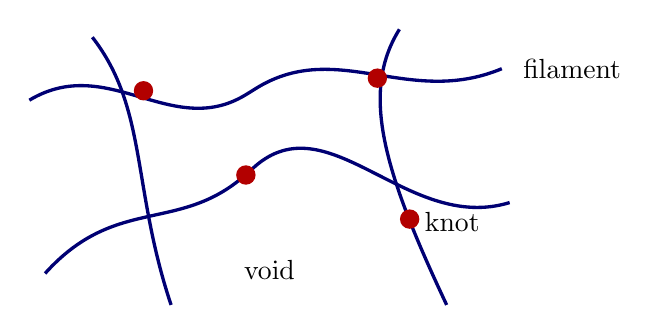
\begin{tikzpicture}[x=1cm,y=1cm]
  \draw[rounded corners=2pt,very thick,blue!45!black]
    (0.2,2.7) .. controls (1.2,3.3) and (2.0,2.2) .. (3.0,2.8)
    .. controls (4.1,3.5) and (5.0,2.6) .. (6.2,3.1);
  \draw[rounded corners=2pt,very thick,blue!45!black]
    (0.4,0.5) .. controls (1.3,1.5) and (2.1,1.0) .. (3.0,1.8)
    .. controls (4.0,2.7) and (5.0,1.0) .. (6.3,1.4);
  \draw[rounded corners=2pt,very thick,blue!45!black]
    (1.0,3.5) .. controls (1.7,2.6) and (1.5,1.6) .. (2.0,0.1);
  \draw[rounded corners=2pt,very thick,blue!45!black]
    (4.9,3.6) .. controls (4.4,2.8) and (4.7,1.8) .. (5.5,0.1);
  \fill[red!70!black] (1.65,2.82) circle (3.5pt);
  \fill[red!70!black] (4.62,2.98) circle (3.5pt);
  \fill[red!70!black] (2.95,1.75) circle (3.5pt);
  \fill[red!70!black] (5.03,1.19) circle (3.5pt);
  \node[align=center] at (3.25,0.55) {void};
  \node[right] at (6.35,3.1) {filament};
  \node[right] at (5.1,1.15) {knot};
\end{tikzpicture}
\caption{Une analogie bidimensionnelle simple du réseau de caustiques : des concentrations filiformes entourent des vides et se rejoignent en des nœuds plus lumineux. En trois dimensions, les plis principaux sont des feuillets dont les intersections forment des filaments et des nœuds.}
\label{fig:c09-caustic-network}
\end{figure}

La construction sans force ne remplace pas la théorie des perturbations cosmologiques. La gravité est essentielle à la croissance des contrastes de densité, à la formation des halos, des galaxies et des structures non linéaires. Le modèle jouet isole un fait géométrique robuste : un flot initial légèrement variable se replie et se concentre naturellement. On pourrait aussi inclure de petites variations initiales de densité sans modifier l’argument central fondé sur le jacobien.

Nous avons donc déplacé le mystère plutôt que de l’éliminer. L’inflation a été introduite pour étirer une région jusqu’à la rendre extraordinairement plate et uniforme. Le calcul des caustiques suppose un champ initial de petites variations de vitesse. D’où vient cette graine inhomogène ? Le prochain cours portera sur les fluctuations quantiques des champs pendant l’inflation et examinera comment elles deviennent les conditions initiales du réseau cosmique ultérieur.

\section{Ce que l’argument a établi}

Un champ scalaire homogène se comporte comme une coordonnée évoluant dans le potentiel \(V(\phi)\). Dans une boîte fixe, il obéit à \(\ddot\phi=-V'(\phi)\). Dans une boîte comobile en expansion, le volume physique \(a^3\) intervient dans l’action et donne
\[
\ddot\phi+3H\dot\phi=-V'(\phi).
\]
Le frottement de Hubble peut maintenir le champ dans un mouvement terminal lent sur un potentiel élevé et peu pentu. Son énergie cinétique devient alors négligeable, son énergie potentielle maintient \(H\) presque constant, et \(a(t)\) croît approximativement de façon exponentielle.

L’expansion dilue les monopôles indésirables, lisse la géométrie et entraîne la courbure vers zéro. Pourtant, l’inflation doit prendre fin. Le champ quitte le plateau, oscille et transfère son énergie aux particules chaudes du réchauffement. Plusieurs questions restent ouvertes : la forme du potentiel, l’identité et l’état initial de l’inflaton, ses couplages responsables du réchauffement et la très faible énergie du vide observée aujourd’hui.

Le succès de l’inflation soulève une dernière question. Un Univers parfaitement lissé ne contiendrait aucune galaxie. L’application caustique
\[
y=x+v(x)t,
\qquad
\frac{dn}{dy}=\frac{1}{1+v'(x)t}
\]
montre comment de petites variations dans un flot initial peuvent engendrer des feuillets, des filaments et des nœuds marqués. Elle n’explique pas l’origine de ces variations. Leur origine quantique est le sujet que nous abordons maintenant.
